\documentclass[12pt]{article}
\usepackage[margin=1in]{geometry}
\usepackage{hyperref}
\usepackage[utf8]{inputenc}
\usepackage{amsmath}
\usepackage{graphicx}
\usepackage{float}
\graphicspath{ {./images/} }
\usepackage{subcaption}
\usepackage{physics}
\setlength{\parskip}{1em}
\usepackage{minted} 
\usepackage{xcolor} % to access the named colour LightGray
\definecolor{LightGray}{gray}{0.9}
\usepackage{indentfirst}
\usepackage{url}
\usepackage{wrapfig}
\title{CTA200 Project}
\author{Isabella Armstrong \\ 1006822967\\
\href{mailto:isabella.armstrong@mail.utoronto.ca}{isabella.armstrong@mail.utoronto.ca}}
\date{\today}
\usepackage{ragged2e}

\begin{document}
\maketitle
\section{Introduction}
The existence of hypervelocity stars (HVS) provide unique insight into the structure of the Milky Way potential. Before studying how hows HVSs are impacted but subtle variations in the Milky Way potential, it is important to understand how they respond to non-subtle changes in the potential. This project uses {\fontfamily{qcr}\selectfont speedystar}(\cite{2017MNRAS.467.1844R}, \cite{2018MNRAS.476.4697M}, \cite{2019MNRAS.487.4025C}, \cite{2022MNRAS.517.3469E}) to propagate and perform photometry on mock HVS populations. Conservation of energy allows a relationship to be derived between the initial velocity, position, and galactic potential and the final velocity, position and potential of the HVS. By varying speedystar input parameters, the effects of the Milky Way halo mass on the HVS population is explored. \par 

For this project, a script {\fontfamily{qcr}\selectfont CTA200Project.py} was written which uses {\fontfamily{qcr}\selectfont speedystar} to create an ejection catalog of HVSs (see \ref{appendix} for installation instructions and trouble shooting). This catalog is then propagated through three different Milk Way potentials each with a different dark matter halo scale factor, creating three different star samples. A propagation.fits file is saved for each potential. A sub-sample of HVS with velocities greater than the escape velocity at their position is selected an photometry is performed, and a photometry.fits files is saved for each sample. \par 

After generating the star samples and saving the necessary information, the .fits files containing the photometry information are read and the total Galactocentric position, velocities (GCv), and the Galactic escape velocity (Vesc) at the HVSs position are saved. Stars with absolute magnitude greater than 20.7 are selected. Plots of Distance vs HVS number and  Vesc vs GCv are made and saved in both .pdf and .png formats.  

\section{Speedystar Structure}
{\fontfamily{qcr}\selectfont speedystar} is a python program which generates mock catalogs of HVSs. It takes in an ejection model, which determines how the spatial and velocity distribution of the stars will be sampled. This project uses the Hills mechanism \cite{1988Natur.331..687H}, implemented in {\fontfamily{qcr}\selectfont speedystar} as {\fontfamily{qcr}\selectfont speedystar.eject.Hills} (\cite{2017MNRAS.467.1844R}, \cite{2018MNRAS.476.4697M}) to generate the catalog and saves the masses, velocities, ages, flight times, luminosity, radii and evolutionary stage of each star.

After the population is generated, a Galactic potential is defined and the star sample is propagated through the Galaxy in 0.1 Myr timesteps. This project uses the Galactic potential {\fontfamily{qcr}\selectfont speedystar.utils.mwpotential} \cite{Evans_2021}, which allows us to vary the Milky Way halo mass.  

After the sample is propagated, mock observations of the ejected stars are obtained. Apparent magnitudes in a variety of bands are saved. The dust map dust-map-3d.h5 is used when computing apparent magnitudes \cite{bovy_2015_31262}. 

\subsection{Milky Way Potential}\label{sec:MWpot}

As stated above, the function {\fontfamily{qcr}\selectfont speedystar.utils.mwpotential} is used to define a Galactic potential. This takes into account contributions from the Milky Way as well as the moving LMC potential. The potential is comprised of several sub components, whose values can be changed. The central massive black hole (MBH) is modeled by the Keplerian potential given in (\ref{eqn:MBH}). 
\begin{equation}\label{eqn:MBH}
    \Phi_{BH,GC}(r) = -G\frac{4\cross10^6M_\odot}{r}
\end{equation}
where r is the Galactocentric distance. 
The Galactic Bulge is modeled by a Hernquist potential given by (\ref{eqn:bulge})\cite{Hernquist} . This model was derived using the de Vaucouleurs profile, and its simple relation between density and potential make it easy to implement \cite{Vaucouleurs}.  

\begin{equation}\label{eqn:bulge}
    \Phi_{Bulge,GC}(r) = -\frac{GM_b}{r+r_b}
\end{equation}

where $M_b = 3.4\cross 10^10 M_\odot$ and $r_b = 0.7$kpc \cite{Price-whelan}. The potential in the galactic disc is given by a Miyamoto-Nagai potential (\ref{eqn:disc}) \cite{Miyamoto}.

\begin{equation}\label{eqn:disc}
    \Phi_{Disc}(R,z) = -\frac{GM_d}{\sqrt{R^2+(a_d+\sqrt{z^2+b_d^2}}}
\end{equation}
here $M_d = 10^{11}M_\odot$ is the disc mass, $a_d = 6.5$kpc is disc scale length and $b_d = 260$pc is disc scale height \cite{Price-whelan}. The values for $M_b$, $r_b$, $M_d$, $a_d$, and $b_d$ were calculated by inferring the Galactic potential with tidal streams and assuming that the dark matter halo is triaxial. \cite{Price-whelan}. The dark matter contribution is give by a spheroidal NFW potential \cite{NFW}. 

\begin{equation}\label{eqn:NFW}
    \Phi_{NFW}(r) =  -\frac{4\pi G\rho_0 R_s^3}{r}\ln\left(1 + \frac{r}{R_s}\right)
\end{equation}
and 
\begin{equation}\label{eqn:NFWRho}
    \rho(x,y,z) = \frac{M_s}{4\pi r_s}\frac{1}{(\zeta/r_s)(1+\zeta/r_s)^2}, \zeta^2 = x^2 + y^2 + \frac{z^2}{c_{halo}}
\end{equation}
where $\rho_0$ is some initial parameter that depends on the scale mass $M_s$. A scale radius of $R_s = 24.8$kpc is taken \cite{Rossi}. We assume a spherical dark matter halo and that $c_{halo} =1$. 

The LMC potenital is comprised of a Keplerian (\ref{eqn:MBH}) plus Hernquist bulge (\ref{eqn:bulge}). A LMC MBH mass of $10^5M_\odot$ is assumed. The scale mass is taken as $M_{LMC} = 1.5\cross 10^{11}M_\odot$ and the scale radius is taken to be $R_{LMC} = 17.14$kpc \cite{Evans_2021}. The initial position of the LMC is take as its observed position and velocity today. The centre-of-mass position is $\alpha = 78.76^{\circ}$, $\delta = -69.19^{\circ}$ \cite{Zivick}, propermotion of $(\mu_\alpha, \mu_\delta) = (1.91,\,0.229)$mas/yr \cite{Kall}, heliocentric distance of 49.97 kpc \cite{Pietrzy}, and radial velocity of +262.2 km/s \cite{van} are used. 

The total potential given by {\fontfamily{qcr}\selectfont speedystar.utils.mwpotential} is the sum individual potential components (\ref{eqn:total-pot}). 
\begin{equation}\label{eqn:total-pot}
    \Phi = \Phi_{BH,GC} + \Phi_{Bulge, GC} + \Phi_{disc} + \Phi_{NFW} + \Phi_{BH,LMC} + \Phi_{Bulge, LMC}
\end{equation}

The default values for {\fontfamily{qcr}\selectfont speedystar.utils.mwpotential} are a NFW scale mass of $M_s = 0.76\cross10^{12}M_\odot$, a radial profile $r_s  = 24.8$kpc, an axis ration of $c=1$, and the $T=True$ so that {\fontfamily{qcr}\selectfont triaxialNFWPotential} is used. 

\section{Conservation of Energy} \label{sec:consE}
%	HVSs are ejected with a velocity v_1 at a distance r_1 from the Galactic Centre, where the strength of the Galactic potential is Phi_1  and after propagation end up with a velocity v_2 at a distance r_2 where the strength of the Galactic potential is Phi_2. Using a conservation of energy argument, express v_2 in terms of v_1, r_1 and r_2 in the Galactic potential implemented by MWPotential. Assume the dark matter halo of MWPotential is spherical and that stars only move along the x-axis of the Galaxy, i.e. r=x, y=0, z=0.

HVSs are initial ejected with velocity $v_1$, at position $r_1$ where the strength of the Galactic potential  is $\Phi_1$. After propagation, they have velocity $v_2$, and position $(r_2)$ where the strength of the potential is $\Phi_2$. Since energy is conserved, a relationship between $v_2$ and the other parameters can be derived. The initial energy of an HVS is given by (\ref{eqn:E1})
\begin{equation}\label{eqn:E1}
    E_1 = \frac{1}{2}mv_1^2 + \Phi_1
\end{equation}
where $m$ is the mass of the HVS. Energy conservation states that $E_1 = E_2$, where $E_2 = \frac{1}{2}mv_2^2 + \Phi_2$. Therefore 
\begin{equation}
    v_2^2 = v_1^2 + \frac{2}{m}\left(\Phi_1 - \Phi_2\right)
\end{equation}
where $\Phi_1$ and $\Phi_2$ are \ref{eqn:total-pot} evaluated at $r_1$ and $r_2$ respectively. 


\section{Effects of Milky Way Halo Mass on HVS Properties}

The value of the scale mass in the Milky Way dark matter halo effects the properties of the observable HVS sample. In order to explore these difference, a HVS ejection catalog was created. An ejection rate of $10^{-3}$ HVS/year was used. This is an order of magnitude larger than the default ejection rate of $10^{-4}$ HVs/year. This was done to improve statistics and better study the differences caused by varying the dark matter halo scale mass $(M_s)$. \par 

The HVS catalog was propagated through three different Milky Way potentials: $M_s = [0.076, 0.76, 1.76]$. A total of 5707 HVSs were propagated through the Milky Way potential. For a HVS to be detectable, its total Galactocentric velocity (GCv) must be greater than the escape velocity to infinity at the star's current position (Vesc). Additionally, it must have magnitude  Gaia$_G$ $<$ 20.7 making it bright enough detect with the Gaia satellite. The number of these potentially detectable HVSs varied with $M_s$. For $M_s = 0.076$, 684 of the 5707 HVSs were detectable. For $M_s = 0.76$ this number was 538 and for $M_s = 1.76$ it was 433. Table (\ref{tab:detectHvs}) summarizes this information. As the mass of the Halo increases, so does the strength of the potential and as a result fewer of the HVS in the initial ejection catalog  reach velocities greater than the escape velocity of the Galaxy after propagation.

\begin{table}[H]
    \centering
    \begin{tabular}{|c|c|c|}
    \hline 
        \textbf{Scale Mass ($M_s$)} & \# of Observable HVS & \% of Ejection Catalog \\
        \hline 
        0.076 & 684 & 12 \\
        \hline
        0.76  & 538 & 9.4\\
        \hline
        1.76 & 433 & 7.6 \\
        \hline
    \end{tabular}
    \caption{The number of observable HVSs and percentage of the original catalog that is observable for each scale mass.}
    \label{tab:detectHvs}
\end{table}

The condition GCv $>$ Vesc removed 20\% of the initial ejection catalog for $M_s = 0.076$ up to 36\% of the initial catalog for $M_s = 1.76$. As $M_s$ increases so does the strength of the potential the ejection catalog is propagated through. Therefore it makes sense that the number of observable HVS decreases as the potential increases. The condition that Gaia$_G$ $<$ 20.7 removed an additional 85\% to 88\% of the remaining HVSs after the velocity condition was applied. Apparent magnitude is the greater limiting factor in observation. Unlike the velocity condition, there was only a $3\%$ difference in the percentage that was removed for the different samples.
\par 
The total Galactocentric distance of the observable HVSs is shown in figure (\ref{fig:GCdist}). Each HVS is assigned a number corresponding to its position in the initial ejection catalog. Different HVSs are observable depending on the value of $M_s$; however, the distribution in position for the three potentials is the same. \par 

As discussed in section \ref{sec:consE}), the final velocity of an HVS depends on its initial velocity, position, and final position, and the strength of the Milky Way potential. Therefore, an HVS that is observable when propagated through the $M_s = 0.076$ potential may not have a great enough velocity of escape the Galaxy when propagated through the $M_s = 1.76$ potential. This also accounts for why a larger percentage of the original ejection catalog is observable for $M_s = 0.076$ when compared to the greater scale factors. \par 

As $M_s$ increases, so does the escape velocity at a fixed Galactocentric velocity (GCv). Figure (\ref{fig:VescVsGCv}) plots GCv versus Vesc for the three simulations and clearly shows how increasing $M_s$ corresponds to an increase in escape velocity.
An increase in $M_s$ corresponds to an increase in the strength of the Milky Way potential (see section \ref{sec:MWpot} equations \ref{eqn:NFW} and \ref{eqn:NFWRho}). 

\begin{figure}[H]
    \centering
    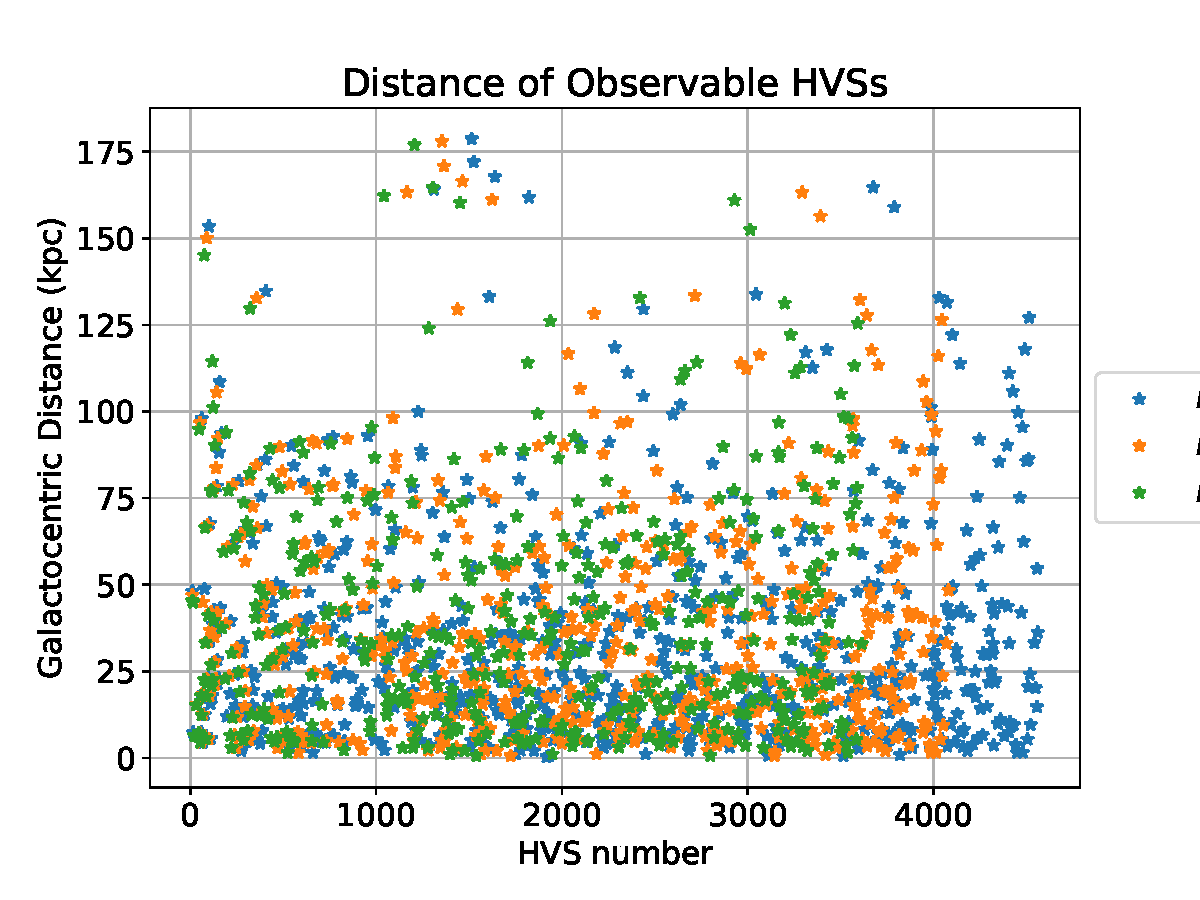
\includegraphics[width=0.85\textwidth]{GCdist.png}
    \caption{Galactocentric total distances in kpc of observable HVSs in the three simulations. After propagation, different HVSs are observable depending on the value of $M_s$.  
    All three samples have the same distribution in GCv.}
    \label{fig:GCdist}
\end{figure}

\begin{figure}[htb]
    \centering
    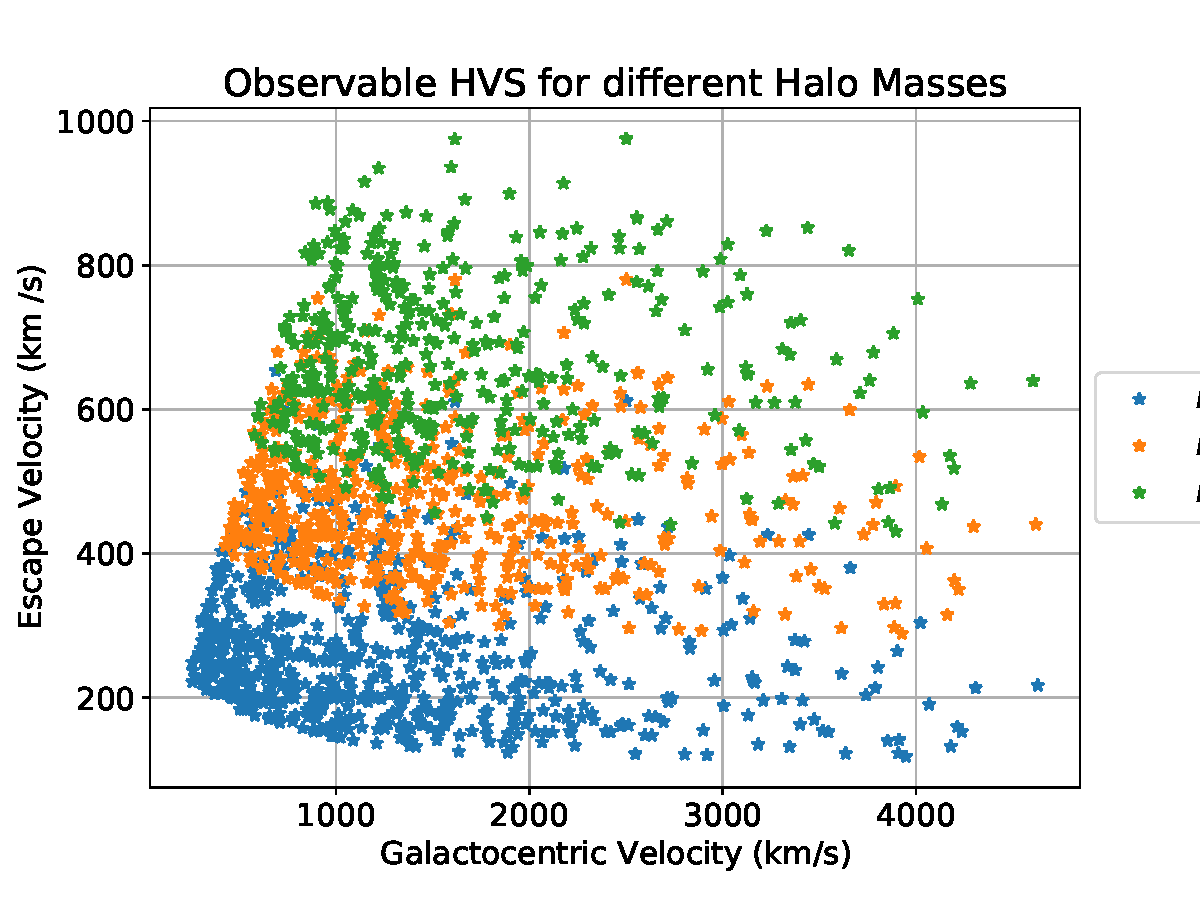
\includegraphics[width=0.85\textwidth]{VescVsGCv.png}
    \caption{Escape Velocity versus total Galactocentric velocity for the three simulations. The blue stars correspond to the least massive halo with $M_s = 0.076$ and have lower escape velocities at a given GCv compared to the Green stars, corresponding to a scale mass of 1.76. The orange stars have $M_s = 0.76$; the default value.}
    \label{fig:VescVsGCv}
\end{figure}




\pagebreak 
%
\section{Appendix}\label{appendix}

{\fontfamily{qcr}\selectfont speedystar} can be downloaded and installed from \url{https://github.com/fraserevans/speedystar}. Some trouble shooting notes 
\begin{itemize}
    \item In line 6 of setup.py there should be a comma after long\textunderscore 
    description 
    \item pygaia has been uploaded since the last release of speedystar. Uninstall pygaia, and pip install pygaia==2.2. If this doesn't work, change line 88 from mysample.photometry() to mysample.photmetry(errors=None). 
    
    \item the dust maps must be downloaded before running. Line 85 of my code calls on speedystar.fetch\textunderscore dust(), which should download the dust maps for you. It didn't work on my installation but it should've. The dustmap I used can be directly downloaded from here \url{https://zenodo.org/record/31262/files/dust-map-3d.h5}
    
    \item A full Amuse installation is required. See \url{https://amuse.readthedocs.io/en/latest/install/howto-install-AMUSE.html#installing-amuse} for more detailed installation instructions if speedystar does not correctly install it the first time 
    \item I initially had trouble with scanninglaw. My code doesn't use it so if a : No module named 'scanninglaw' asrise, you can comment out the line 12 in \textunderscore\textunderscore init\textunderscore\textunderscore .py and hopefully my code will run.
    \item Let me (or Fraser fraser.evans@utoronto.ca) know if any other issues arise.
\end{itemize}

\section*{}\label{refrences}

\bibliographystyle{abbrv}
\bibliography{bib}


\end{document}
